%%%%%%%%%%%%%%%%%%%%%%%%%%%%%%%%%%%%%%%%%
% Beamer Presentation
% LaTeX Template
% Version 1.0 (10/11/12)
%
% This template has been downloaded from:
% http://www.LaTeXTemplates.com
%
% License:
% CC BY-NC-SA 3.0 (http://creativecommons.org/licenses/by-nc-sa/3.0/)
%
%%%%%%%%%%%%%%%%%%%%%%%%%%%%%%%%%%%%%%%%%

%----------------------------------------------------------------------------------------
%	PACKAGES AND THEMES
%----------------------------------------------------------------------------------------

\documentclass{beamer}
\usepackage{subcaption}

\mode<presentation> {
	
	% The Beamer class comes with a number of default slide themes
	% which change the colors and layouts of slides. Below this is a list
	% of all the themes, uncomment each in turn to see what they look like.
	
	%\usetheme{default}
	%\usetheme{AnnArbor}
	%\usetheme{Antibes} %three-row header
	%\usetheme{Bergen} %side
	%\usetheme{Berkeley} %side
	%\usetheme{Berlin} %dots by sub + subsec header
	%\usetheme[secheader]{Boadilla} % maybe
	%\usetheme{Boadilla} % maybe
	%\usetheme{CambridgeUS}
	%\usetheme{Copenhagen} %heavy sec+subsec header
	%\usetheme{Darmstadt} % dots by sec + subsec header
	%\usetheme{Dresden} % maybe
	\usetheme{Frankfurt} % maybe % dots by sec 
	%\usetheme{Goettingen}
	%\usetheme{Hannover}
	%\usetheme{Ilmenau}
	%\usetheme{JuanLesPins}
	%\usetheme{Luebeck}
	%\usetheme{Madrid} % maybe
	%\usetheme{Malmoe}
	%\usetheme{Marburg}
	%\usetheme{Montpellier}
	%\usetheme{PaloAlto}
	%\usetheme{Pittsburgh}
	%\usetheme{Rochester}
	%\usetheme{Singapore} % maybe
	%\usetheme{Szeged}
	%\usetheme{Warsaw}
	
	% As well as themes, the Beamer class has a number of color themes
	% for any slide theme. Uncomment each of these in turn to see how it
	% changes the colors of your current slide theme.
	
	%\usecolortheme{albatross}
	%\usecolortheme{beaver} % rosso
	%\usecolortheme{beetle}
	%\usecolortheme{crane}
	%\usecolortheme{dolphin} % viola
	%\usecolortheme{dove}
	%\usecolortheme{fly}
	%\usecolortheme{lily} % viola, se fosse rosso...
	%\usecolortheme{orchid}
	%\usecolortheme{rose}
	%\usecolortheme{seagull}
	%\usecolortheme{seahorse}
	\usecolortheme{whale}
    %\usecolortheme{wolverine}
	
	%\setbeamertemplate{footline} % To remove the footer line in all slides uncomment this line
	%\setbeamertemplate{footline}[page number] % To replace the footer line in all slides with a simple slide count uncomment this line
	
	\setbeamertemplate{navigation symbols}{} % To remove the navigation symbols from the bottom of all slides uncomment this line
	
}

\usepackage{graphicx} % Allows including images
\usepackage{booktabs} % Allows the use of \toprule, \midrule and \bottomrule in tables
%\usepackage{enumitem}

%----------------------------------------------------------------------------------------
%	TITLE PAGE
%----------------------------------------------------------------------------------------

\title[Seismic Time Series Analysis]{Seismic Time Series Analysis} % The short title appears at the bottom of every slide, the full title is only on the title page

\author{Marco Ciotola} % Your name
\institute[Ca' Foscari] % Your institution as it will appear on the bottom of every slide, may be shorthand to save space
{
	Ca' Foscari University\\ % Your institution for the title page
	\medskip
	\textit{848222@stud.unive.it} % Your email address
}
\date{June 16, 2020} % Date, can be changed to a custom date

\begin{document}
	

\begin{frame}[plain,noframenumbering]
	\titlepage % Print the title page as the first slide
\end{frame}

%----------------------------------------------------------------------------------------
%	PRESENTATION SLIDES
%----------------------------------------------------------------------------------------

%------------------------------------------------
\section{Introduction} % Sections can be created in order to organize your presentation into discrete blocks, all sections and subsections are automatically printed in the table of contents as an overview of the talk
%------------------------------------------------
\subsection{Goal}
\begin{frame}{Lockdown influence on seismic surveys}
	\begin{columns}[c]
		\column{0.666\textwidth}
		\centering\large COVID-19 outbreak\\
		\vspace{.5em}\centering\large$\Downarrow$\vspace{.5em}\\
		\centering\large Lockdown\\\small(March $14^{th}$, 2020) \\
		\vspace{.5em}\centering\large$\Downarrow$\vspace{.5em}\\
		\centering\large \textbf{Influence on background noise}\\
		\vspace{.5em}\centering\large$\Downarrow$\vspace{.5em}\\
		\centering\large \textit{Human activity correlation}\note{Our study cannot fulfill this point} \\
	\end{columns}
\end{frame}

\subsection{Dataset}

\begin{frame}{Data source}
	\begin{columns}[c]
		\column{0.666\textwidth}
		\begin{columns}[c]
			\column{0.13\textwidth}
			\column{0.2\textwidth}
			\begin{figure}
				
\includegraphics[width=\linewidth,clip=true]{slides_files/ROB-logo}
			\end{figure}
			\column{0.57\textwidth}\vspace{.4em}\\
			\small Royal Observatory of Belgium\\\scriptsize\textit{Seismology-Gravimetry}
			\column{0.1\textwidth}
		\end{columns}
		\begin{figure}
			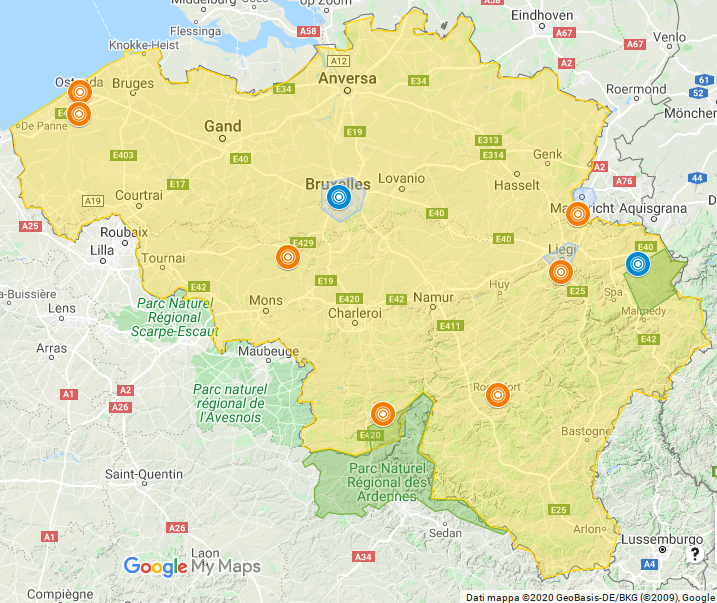
\includegraphics[width=.8\linewidth]{slides_files/stations-map-smol-2}
		\end{figure}
		\column{0.3\textwidth}
		\centering 9 stations
		\\\vspace{.3em}$\downarrow$
		\\\vspace{.3em}2 selected
		\\~\\~
		\\\vspace{.25em}\textbf{Uccle}\\in Brussels\\~
		\\\vspace{.25em}\textbf{Membach}\\mountain area\\near a national park\\~
		\column{0.033\textwidth}
	\end{columns}
\end{frame}

\begin{frame}{Data description}
	\begin{columns}[T]
		\column{.5\textwidth}
		(min, max) displacements\hfill$\rightarrow$\\~\\
		second precision\hfill$\rightarrow$\\~\\
		UTC times\hfill$\rightarrow$\\~\\
		missing values\hfill$\rightarrow$
		\column{.5\textwidth}
		total displacement (difference)\\~\\
		hourly mean\\~\\
		legal-time conversion\\~\\
		fill with weekly mean\\(when needed)
	\end{columns}
\end{frame}

\begin{frame}{Dataset division}\centering
	%Data from October $29^{th}$, 2018 to April $27^{th}$ 2020\\~\\
	We want to be able to verify our models on pre-lockdown data
	\vspace{0.1\textheight}
	\begin{columns}
		\column{0.90\textwidth}
		\begin{columns}
			\column{0.54\textwidth}\hspace{-.005\textwidth}29-10-2018\\\hspace{-.005\textwidth}\tiny$\vert$
			\column{0.255\textwidth}\centering
			28-10-2019\\\tiny$\vert$
			\column{0.205\textwidth}\centering
			02-03-2020\\\tiny$\vert$
		\end{columns}
		\begin{columns}
			\column{0.6667\textwidth}$\underbrace{\rule[.5em]{\textwidth}{0.15em}}$
			\column{0.2307\textwidth}$\underbrace{\rule[.5em]{\textwidth}{0.15em}}$
			\column{0.1026\textwidth}$\underbrace{\rule[.5em]{\textwidth}{0.15em}}$
		\end{columns}
		\begin{columns}
			\column{0.6667\textwidth}\centering
			Training set - \textbf{67\%}
			\column{0.2307\textwidth}\centering
			\hspace{-.3em}Test set - \textbf{23\%}\hspace{-.3em}
			\column{0.1026\textwidth}\centering
			\textbf{10\%}
		\end{columns}
	\end{columns}
	\vspace{0.1\textheight}
	Fit on training $\rightarrow$ validate on test $\rightarrow$ assess lockdown influence
\end{frame}

%------------------------------------------------
\section{Initial analysis}
%------------------------------------------------

\subsection{Seasonality}
\begin{frame}{\subsecname~- Visual inspection}
	\centering Plot review\\
	$\Downarrow$\\ %hints
	Daily and weekly seasonalities\\~
	\begin{figure}
		\begin{subfigure}{.49\linewidth}
			\includegraphics[width=\linewidth]{"project.uccs_files/figure-latex/whole data plot-2"}
		\end{subfigure}
		\begin{subfigure}{.49\linewidth}
			\includegraphics[width=\linewidth]{"project.mems_files/figure-latex/whole data plot-2"}
		\end{subfigure}
		\caption{Zoom from January $6^{th}$ to February $3^{rd}$ 2019}
	\end{figure}
\end{frame}

\begin{frame}{\subsecname~- Periodgram}
	\centering Fourier Transform with different frequencies\\
	$\Downarrow$\\ %reveals
	Daily and weekly seasonalities\\~
	\begin{figure}
		\begin{subfigure}{.49\linewidth}
			\includegraphics[width=\linewidth]{"project.uccs_files/figure-latex/periodgram-1"}
		\end{subfigure}
		\begin{subfigure}{.49\linewidth}
			\includegraphics[width=\linewidth]{"project.mems_files/figure-latex/periodgram-1"}
		\end{subfigure}
	\end{figure}
\end{frame}

\subsection{Decomposition}
\begin{frame}{\subsecname~- Trend extraction}\centering
	Tested simple, Spencer's and Moving Average filters
	\begin{figure}
		\includegraphics[width=.6\linewidth]{"project.uccs_files/figure-latex/trend MA-2"}
	\end{figure}
	\large$\Downarrow$\\\normalsize\textbf{Moving Average}\\\small better seasonal features
\end{frame}

\begin{frame}{\subsecname~- Seasonality extraction}
	\centering MA filter for detrending\\+\\local mean method%\\
%	single \& multiple seasonalities extraction
	\begin{figure}
		\begin{subfigure}{.49\linewidth}
			\includegraphics[width=\linewidth]{"project.uccs_files/figure-latex/extract both 24 and 168-2"}
			\caption{Uccle, Brussels}
		\end{subfigure}
		\begin{subfigure}{.49\linewidth}
			\includegraphics[width=\linewidth]{"project.mems_files/figure-latex/extract both 24 and 168-2"}
			\caption{Membach}
		\end{subfigure}
	\end{figure}
	\large$\Downarrow$\\
	\normalsize\textbf{Only weekly seasonality}\\\small fitting models
\end{frame}

%------------------------------------------------
\section{Parameters estimation}
%------------------------------------------------
\subsection{Uccle}

\begin{frame}{\subsecname~- ARMA orders}
	\begin{figure}[h]
		\centering
		\caption{ACF and PACF plots after \textit{diff} at lag 168}
		\includegraphics[width=0.7\linewidth]{"project.uccs_files/figure-latex/diffs/d168-acf-pacf-1"}
	\end{figure}
	\begin{columns}
		\column{.22\linewidth}
		\column{.28\linewidth}\centering
		$\Downarrow$\\
		non-seasonal AR\\
		order 2
		\column{.38\linewidth}\centering
		$\Downarrow$\\
		seasonal MA\\
		order 1
		\column{.12\linewidth}
	\end{columns}~\\~
%	\centering	This hints to $\mathrm{ARIMA}(2,0,0)(0,1,1)_{168}$
\end{frame}

\begin{frame}{\subsecname~- Remaining seasonality}
	\centering
	ACF and PACF plots highlight 24-hours seasonality on residuals\\~
	\begin{figure}[h]
		\centering
		\includegraphics[width=0.7\linewidth]{"project.uccs_files/figure-latex/arima-35"}
	\end{figure}
\end{frame}

\begin{frame}{\subsecname~- Models comparison}
	\begin{table}
		\begin{tabular}{c | c c c}
%			\toprule
			               &     & (refit) & Box-Pierce \\
			\textbf{ARIMA} & AIC & MAPE    & p-value \\
			\midrule
			$(2,0,0)(0,1,1)_{168}$ & 119700.1 & 5.89\% & 0.333 \\
			$(3,1,1)(0,1,1)_{168}$ & 119513.4 & 6.10\% & 0.854 \\
			$(4,1,2)(0,1,1)_{168}$ & 119396.9 & 6.13\% & 0.109\\
%			\bottomrule
		\end{tabular}
	\end{table}
	\vspace{0.1\textheight}\centering
	Other models have higher AIC and MAPE, while p-value $< 0.05$
\end{frame}

\begin{frame}{\subsecname~- Models validation}
	\begin{figure}
		\begin{subfigure}{.49\linewidth}
			\includegraphics[width=\linewidth]{"project.uccs_files/figure-latex/arima-37"}
		\end{subfigure}
		\begin{subfigure}{.49\linewidth}
			\includegraphics[width=\linewidth]{"project.uccs_files/figure-latex/arima-69"}
		\end{subfigure}
	\end{figure}
	\begin{columns}[T]
		\column{.28\linewidth}\raggedleft~\\~\\\vspace{1em}accepted model $\Rightarrow$\hspace{-1.3em}
		\column{.72\linewidth}
		\begin{table}
			\begin{tabular}{c | c c c}
				%			\toprule
				\textbf{ARIMA} & MAPE   & 80\% CI & 95\% CI \\
				\midrule
				$\mathbf{(2,0,0)(0,1,1)_{168}}$ & 17.48\% & $\approx81\%$ & $\approx91\%$ \\
				$(3,1,1)(0,1,1)_{168}$ & 15.18\% & $\approx96\%$ & $\approx98\%$ \\
				$(4,1,2)(0,1,1)_{168}$ & 14.68\% & $\approx98\%$ & $\approx99\%$ \\
				%			\bottomrule
			\end{tabular}
		\end{table}
		\column{.05\linewidth}
	\end{columns}
\end{frame}

\subsection{Membach}

\begin{frame}{\subsecname~- Data transformation}\centering
	Spikes in data make it heavily non-Normal\\$\Downarrow$\\
	Transform using Box-Cox with $\lambda\approx-1$\\ %\quad\Rightarrow\quad y'=(y-1)/y$\\
	\vspace{.5em}\small Safe since all our data is positive\\\vspace{1em}\large$\Downarrow$\vspace{.5em}\\
	\begin{figure}
		\begin{subfigure}{.49\linewidth}
			\includegraphics[width=\linewidth]{"project.mems_files/figure-latex/training data transformation plots-7"}
		\end{subfigure}
		\begin{subfigure}{.49\linewidth}
			\includegraphics[width=\linewidth]{"project.mems_files/figure-latex/training data transformation plots-9"}
		\end{subfigure}
	\end{figure}
\end{frame}

\begin{frame}{\subsecname~- Models validation}
	\begin{figure}
		\begin{subfigure}{.49\linewidth}
			\includegraphics[width=\linewidth]{"project.mems_files/figure-latex/arima-21"}
		\end{subfigure}
		\begin{subfigure}{.49\linewidth}
			\includegraphics[width=\linewidth]{"project.mems_files/figure-latex/arima-13"}
		\end{subfigure}
	\end{figure}
	\begin{columns}[T]
		\column{.28\linewidth}\raggedleft~\\~\\~\\~\\\vspace{1em}accepted model $\Rightarrow$ \hspace{-1.5em}
		\column{.72\linewidth}
		\begin{table}
			\begin{tabular}{c | c c c}
				%			\toprule
				\textbf{ARIMA} & MAPE   & 80\% CI & 95\% CI \\
				\midrule
				$(0,1,0)(0,1,1)_{168}$ & 17.25\% & $\approx99\%$ & $100\%$ \\
				$(0,1,1)(0,1,1)_{168}$ & 17.98\% & $\approx98\%$ & $\approx99\%$ \\
				$\mathbf{(2,0,0)(0,1,1)_{168}}$ & 16.14\% & $\approx73\%$ & $\approx89\%$ \\
				%			\bottomrule
			\end{tabular}
		\end{table}
		\column{.05\linewidth}
	\end{columns}
\end{frame}

%------------------------------------------------
\section{Lockdown impact}
%------------------------------------------------

\subsection{Seasonalities}

\begin{frame}{Multiple seasonalities}\centering
	Seasonalities extracted together
	\begin{figure}
		\begin{subfigure}{.49\linewidth}
			\includegraphics[width=\linewidth]{"project.uccs_files/figure-latex/seasonalities/before-after-compare-1"}
			\caption{Uccle, Brussels}
		\end{subfigure}
		\begin{subfigure}{.49\linewidth}
			\includegraphics[width=\linewidth]{"project.mems_files/figure-latex/seasonalities/before-after-compare-1"}
			\caption{Membach}
		\end{subfigure}
	\end{figure}
	\large$\Downarrow$\\
	\normalsize No significant difference
\end{frame}

\begin{frame}{Weekly seasonality}\centering
	Only weekly seasonality extracted
	\begin{figure}
		\begin{subfigure}{.49\linewidth}
			\includegraphics[width=\linewidth]{"project.mems_files/figure-latex/seasonalities/seasonplot-mean-sd-1"}
		\end{subfigure}
		\begin{subfigure}{.49\linewidth}
			\includegraphics[width=\linewidth]{"project.mems_files/figure-latex/seasonalities/seasonplot-mean-sd-2"}
		\end{subfigure}
	\end{figure}
	\large$\Downarrow$\\
	\vspace{.3em}\normalsize Monday to Friday lower values\\
	\vspace{.3em}Overall flattening towards 0
\end{frame}

\subsection{Forecasts}

\begin{frame}{Forecasts assessment}
	\begin{columns}[c]
		\column{.5\linewidth}
		\begin{figure}
			\includegraphics[width=\linewidth]{"project.uccs_files/figure-latex/final-model-5"}
		\end{figure}
		\begin{figure}
			\includegraphics[width=\linewidth]{"project.uccs_files/figure-latex/final-model-10"}
		\end{figure}
		\column{.5\linewidth}\centering
		\textbf{Uccle, Brussels}\\
		lockdown $\rightarrow$ during lockdown\\~\\
		\begin{columns}[T]
			\column{.2\linewidth}
			\column{.33\linewidth}\raggedleft
			\textbf{MAPE}\\\textbf{80\% CI}\\\textbf{95\% CI}\\
			\column{.2\linewidth}\raggedleft
			${16\%} \rightarrow$\\
			${73\%} \rightarrow$\\
			${89\%} \rightarrow$\\
			\column{.1\linewidth}\raggedright
			$46\%$\\
			$39\%$\\
			$63\%$\\
			\column{.27\linewidth}
		\end{columns}~\\
		$\Downarrow$\\
		Performance degradation
	\end{columns}
\end{frame}

\begin{frame}{Forecasts assessment}
	\begin{columns}[c]
		\column{.5\linewidth}
		\begin{figure}
			\includegraphics[width=\linewidth]{"project.mems_files/figure-latex/final-model-5"}
		\end{figure}
		\begin{figure}
			\includegraphics[width=\linewidth]{"project.mems_files/figure-latex/final-model-10"}
		\end{figure}
		\column{.5\linewidth}\centering
		\textbf{Membach}\\
		lockdown $\rightarrow$ during lockdown\\~\\
		\begin{columns}[T]
		\column{.2\linewidth}
			\column{.33\linewidth}\raggedleft
			\textbf{MAPE}\\\textbf{80\% CI}\\\textbf{95\% CI}\\
			\column{.2\linewidth}\raggedleft
			$17\% \rightarrow$\\
			$81\% \rightarrow$\\
			$91\% \rightarrow$\\
			\column{.1\linewidth}\raggedright
			${14\%}$\\
			${82\%}$\\
			${96\%}$\\
			\column{.27\linewidth}
		\end{columns}~\\
		$\Downarrow$\\
		Slight performance improvement\\
		\textit{lower peaks}
	\end{columns}
\end{frame}


\begin{frame}<0>[noframenumbering]{Models performance}
	\centering Different stations behaviour\\before lockdown $\rightarrow$ during lockdown\\~\\
	\begin{columns}[T]
		\column{.12\linewidth}
		\column{.3\linewidth}\centering
		\textbf{Uccle, Brussels}~~~
		\column{.15\linewidth}\centering
		\column{.35\linewidth}\centering
		\textbf{Membach}
		\column{.08\linewidth}
	\end{columns}
	\begin{columns}[T]
		\column{.12\linewidth}
		\column{.15\linewidth}\raggedleft
		${16\%} \rightarrow$\\
		${73\%} \rightarrow$\\
		${89\%} \rightarrow$\\
		\column{.12\linewidth}\raggedright
		$46\%$\\
		$39\%$\\
		$63\%$\\
		\column{.21\linewidth}\centering
		\textbf{$<$ MAPE $>$}\\\textbf{$<$ 80\% CI $>$}\\\textbf{$<$ 95\% CI $>$}\\
		\column{.17\linewidth}\raggedleft
		$17\% \rightarrow$\\
		$81\% \rightarrow$\\
		$91\% \rightarrow$\\
		\column{.15\linewidth}\raggedright
		${14\%}$\\
		${82\%}$\\
		${96\%}$\\
		\column{.08\linewidth}
	\end{columns}~\\
	\begin{columns}[T]
		\column{.5\linewidth}\centering
		$\Downarrow$\\
		Performance degradation
		\column{.5\linewidth}\centering
		$\Downarrow$\\
		Slight performance improvement\\
		\textit{lower peaks}
	\end{columns}
\end{frame}


%------------------------------------------------
\section{Conclusion}
%------------------------------------------------
\subsection{Models}

\begin{frame}{Models performance}
	- Periodgrams and models confirm \textbf{weekly} and \textbf{daily seasonality}

	~

	- Both chosen models have \textbf{interesting forecasting power}

	~ ~ \textit{Missed daily seasonality}

	~

	- Models have \textbf{same number of parameters} for each component

	~ ~ \textit{Membach data is transformed}

	~

	- Stable \textbf{seasonality explains most of the variability}

	~ ~ \textit{Membach peaks not explained}
\end{frame}

\begin{frame}{Lockdown influence}
	Mixed findings:

	~

	~ - Influence results \textbf{non-significant on seasonality}

	~

	~ - Influence on forecasts \textbf{depends on the station}

	~ ~ ~ \textit{Correlation with station location}

\end{frame}

\subsection{Future Works}
\begin{frame}{Future Works}
	- Models with \textbf{multiple seasonality} components

	~ ~ \textit{MSTL, TBATS, ARIMA with Fourier Terms, ...}

	~

	- Analysis on the other \textbf{7 stations}

	~

	- Analysis when \textbf{$\mathbf{> 2}$ years} of data available

	~

	- Different factors modify \textbf{lockdown impact}

	~ ~ \textit{Location, dimension of nearest city, ...}
\end{frame}

\title{Thank you for your attention}
\date{}
\author{}
\institute{}
\begin{frame}[plain,noframenumbering]
	\titlepage
\end{frame}
	
\end{document} 